\subsection{Orientering af SIFT punkter}
Formålet ved dette skridt er at tildele hvert punkt en orientering.
\\
\\
Et $16\times 16$ dataindsamlingsvindue placeres på interessepunktets skalabillede, omkring interessepunktet. For alle punkter i dataindsamlingsvinduet, er størrelsen af punkternes gradient, og deres orientering beregnet ved:
\begin{equation}
m(x,y) = \sqrt{(L(x + 1, y) - L(x - 1, y))^2 + (L(x, y + 1) - L(x, y - 1))^2} 
\label{magnitudepoint}
\end{equation}
\begin{equation}o(x,y) = tan^{-1}((L(x,y+1) - L(x,y-1))/(L(x+1, y) - L(x-1, y))) 
\label{orientationpoint}
\end{equation}
hvor $m$ er størrelsen af en gradient, og $o$ er gradientens retning. For alle punkter indenfor dataindsamlingsvinduet, udregnes ligning
\eqref{magnitudepoint}, \eqref{orientationpoint}, og danner et gradientvindue $g$ og orienteringsvindue $v$, begge vinduer af størrelse $16\times16$. Gradientvinduet skal herefter foldes med et Gaussisk filter hvor $\sigma_{Gauss} = 1.5 \cdot \sigma_{point}$, med størrelse $16\times16$. Dette udføres for at vægte gradienter nær punktet højere end punkter i udkanten af vinduet.  $\sigma_{Gauss}$ er sigmaværdien tilhørende Gaussfiltret, der foldes med gradientvinduet. $\sigma_{point}$ er sigmaværdien i $DoG$ billedet, punktet er fundet på. 
\\
\\
Der oprettes derefter et orienteringshistogram $H$, med 36 indgange. Orienteringerne angivet i $v$ skal tilføjes histogrammet, vægtet af gradientstyrken angivet i $g$. En indgang i $H$, dækker en vinkel på $10^{\circ}$. F.eks. skal alle gradienter med vinkler mellem  $0^{\circ}-10^{\circ}$, tilføjes vægtet, til $H_1$, osv. Dette resulterer i et orienteringshistogram, hvor indgangen i histogrammet, med størst værdi, bliver bearbejdet. Lowe foreslår, at alle indgange i histogrammet, der ligger indenfor 80\% af det højeste punkt, bliver nye features - dette er undladt her, for at reducere antallet af features. 
\\
Der skal nu foretages en interpolation, omkring den indgang i histogrammet, med størst værdi, for at få et mere præcist estimat af $\theta$. Toppunktet af andengradspolynomiet vil udgøre orienteringen der tildeles punktet. 
\begin{figure}[H]
    \centering
    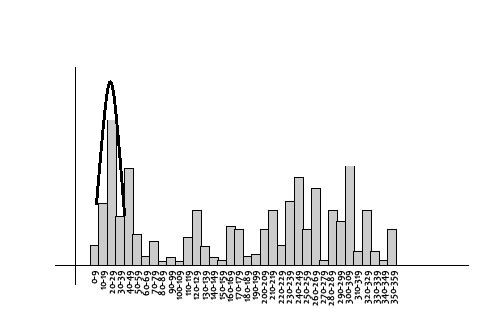
\includegraphics[width=0.60\textwidth]{fig/sift-orientation-histogram.jpg}
     \vspace{-1em}
    \begin{center}    
       \caption{{\footnotesize \textit{Histogrammet $H$ afbilledet, sammen med en andengradsligning. Andengradsligningen er beregnet over den største indgang i $H$}}}
    \label{histogramheight}
     \end{center}
     \vspace{-2.5em}
  \end{figure} \noindent
Dette ses på figur \ref{histogramheight}, hvor et andengradspolynomium er blevet tilnærmet den største værdi af $H$. Estimering af andengradspolynomiet sker over den største værdi i $H$, og dens venstre og højre nabo.


\subsubsection*{Algoritme: SIFT Orientering}
\begin{tabbing}
Input\quad \= : \= Billede $I$\\
$\text{ }$ \> : \> Interessepunkter $p  \in (x, y)$ \\
Output $\text{ }$ \> : \> Interessepunkter tildelt orientering $p \in (x,y, \theta)$
\end{tabbing}
\begin{enumerate}
\item Et dataindsamlingsvindue placeres omkring interessepunktet, på det skalabillede interessepunktet er fundet på.
\item Ligning \eqref{magnitudepoint}, \eqref{orientationpoint} anvendes på hvert punkt i dataindsamlingsvinduet, for at udregne gradient retninger og størrelser. Gradientbilledet foldes derefter med et Gaussisk filter, hvor $\sigma_{Gauss} = 1.5 \cdot \sigma_{point}$
\item Værdierne i $g$ adderes på indgange i histogrammet $H$, afhængigt af deres orientering i $v$.
\item  Der udføres en interpolation omkring den største værdi i $H$ og to naboer. Denne værdi returneres.
\end{enumerate}
